\chapter{Problem Statement} \label{chap:problem_statement} \minitoc

\section*{}

This chapter describes the problem, as it can be seen in Section \ref{sec:current_issues}. In Section \ref{sec:desiderata} it is presented the wanted features for the proposed solution and in Section \ref{sec:scope} the scope of the project is defined. Section \ref{sec:research_questions}contains the research questions to be answered by this dissertation. The experimental methodology is outlined in Section \ref{sec:exp_meth}. Chapter \ref{sec:planning} contains a Gantt chart with a planning of this dissertation. Finally, this chapter is summarized by Section \ref{sec:stat_summary} with an overview of the topics mentioned before.

\section{Current Issues}\label{sec:current_issues}

Chapter \ref{chap:sota} contains several solutions that provide decentralized architecture in visual programming tools applied to the internet of things paradigm. However, some of this tools are specific to a certain paradigm, like Smart Cities or industry. \textcolor{red}{Check this after SOTA}
We can define the problem in these issues:
\begin{enumerate}
    \item \textbf{Discovery of computation capabilities}: the current work lacks the automatic discovery of the computational capabilities of the devices in the network. This information is normally manually introduced by the developer.
    \item \textbf{Leveraging devices in the network}: since most tools use a centralized architecture, including Node-RED, they do not leverage the devices in the network. Fog Computing introduces a decentralized solution, one that can be applied to Node-RED by distributing the computational tasks across the edge devices.
    \item \textbf{Communicate computational capabilities}: current tools require the developer to manually introduce the resources of each device in the network, which is not a scalable solution. This information is vital for the successful distribution of computation across the devices.
    \item \textbf{Detecting non-availability}: when a device fails or becomes unavailable, it is important for the system to automatically realize and adapt. The majority of current solutions do not possess this feature, which is vital if a system aims to dynamically adapt to changes in the environment.
\end{enumerate}

\section{Desiderata}\label{sec:desiderata}

Desiderata is a Latin word that translates to "\emph{things wanted}". In the context of this document, this section contains requirements wanted in a solution that aims to solve all the issues identified in Section \ref{sec:current_issues}. The requirements are the following:

\begin{description}
    \item [D1: Communicate computational capabilities of devices connected] so that this information can be sent to an orchestrator that will decompose the total computation workload based on this data.
    \item [D2: Decomposition and partition of computation] so that the total computational requested can be distributed through all the devices in the network, using information about the computational capabilities and availability of the devices in the network.
    \item [D3: Convert computational tasks into runnable code] so that each computational task can be executed in edge and fog devices, which contain limited resources.
    \item [D4: Provide self-adaptation of the system] so that it can adapt to non-availability of resources or even appearances of new devices.
\end{description}

\section{Scope}\label{sec:scope}

The focus of this dissertation is the development of a prototype that allows for a decentralized orchestration of an IoT system. Despite security being a critical feature, it is considered a secondary goal, allowing the dissertation to focus on the its primary goals.

\textcolor{red}{\textbf{O que coloco mais?}}

%\section{Use Cases}\label{sec:use_cases}

\section{Main Hypothesis}\label{sec:stat_research_questions}

\textcolor{blue}{Write main hypothesis}

This dissertation is built around the following hypothesis:

\textit{Is a decentralized system ... more robust and efficient than a centralized one?}

\section{Experimental Methodology}\label{sec:exp_meth}

In the interest of validating whether or not the solution implemented achieves the \emph{desiderata} and solves the current issues, there will be developed two test scenarios, the first one in a smaller scale and the second in a bigger one, with the use of simulations. Each one of the test scenarios will be verified against each \emph{desiderata}. 

\textcolor{red}{Check if ok}

\section{Planning}\label{sec:planning}

In order to help managing the amount of work needed in the next few months, a \textit{Gantt Chart} was built. It is possible to consult it in Figure \ref{fig:gantt}. 
\begin{figure}[h]
    \caption{\textit{Gantt Chart} for this dissertation}
    \label{fig:gantt}
    \centering
    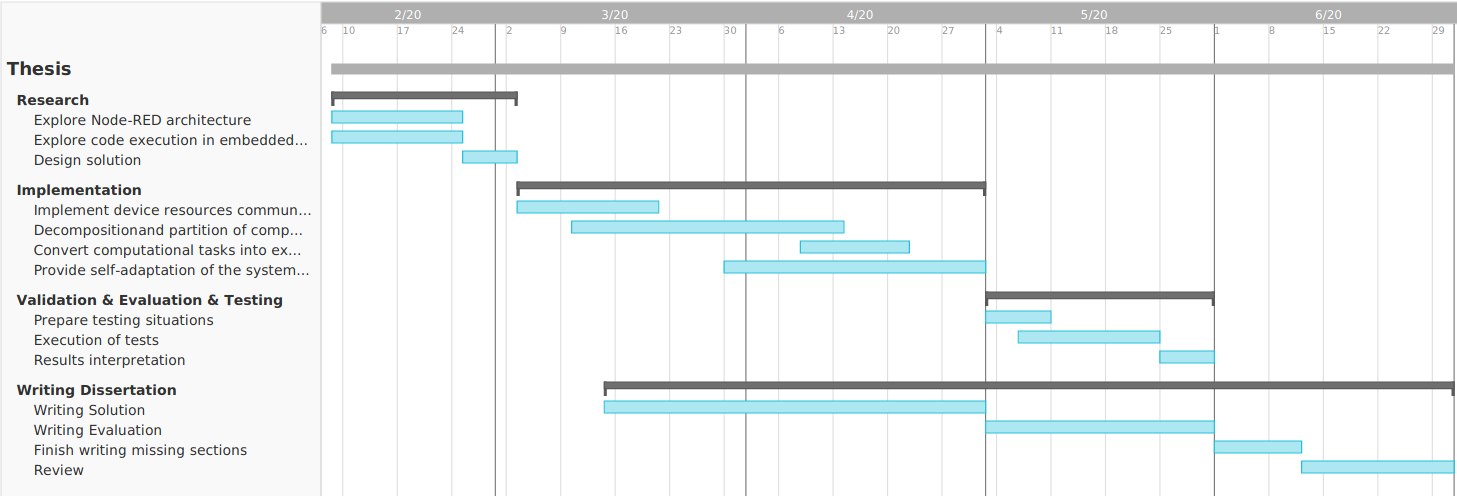
\includegraphics[width=1\textwidth]{gantt_chart.png}
    \end{figure}

\section{Summary}\label{sec:stat_summary}

\textcolor{yellow}{\textbf{**TODO**}}
